\documentclass[journal]{IEEEtran}

\usepackage{amsmath,amssymb,amsfonts}
\usepackage{algorithmic}
\usepackage{graphicx}
\usepackage{textcomp}
\usepackage{xcolor}
\usepackage{booktabs}
\usepackage{microtype}
\usepackage{url}
\usepackage{cite}
\usepackage{hyperref}

\hypersetup{
    colorlinks=true,
    linkcolor=blue,
    citecolor=blue,
    urlcolor=blue
}

\begin{document}

\title{Empirical Evaluation of Adversarial Robustness and Cache Efficiency in Modern In-Place and Adaptive Sorting Algorithms}

\author{Premanth~K.,~\IEEEmembership{Graduate Student Member,~IEEE,}
        and~Co-Authors%
\thanks{Premanth K. is with the Department of Computer Science and Engineering. (e-mail: author@university.edu). Manuscript received November 2026.}}

\markboth{IEEE Transactions on Reliability / Journal of Systems Architecture,~Vol.~XX, No.~X, November~2026}%
{Premanth \MakeLowercase{\textit{et al.}}: Adversarial Robustness and Cache Efficiency in Modern Sorting}

\maketitle

\begin{abstract}
Standard runtime libraries frequently employ introspective or adaptive sorting algorithms under the implicit assumption that average-case performance generalizes across real-world workloads. However, when deployed in security-critical or latency-sensitive systems, sorting kernels remain exposed to algorithmic denial-of-service (DoS) vulnerabilities, duplicate-key stagnation, and branch misprediction cliffs induced by non-uniform data topologies. This paper presents an extensive empirical evaluation of adversarial robustness, operational instruction counts, and cache-scaling behavior across ten contemporary sorting paradigms: \texttt{std::sort} (libstdc++ Introsort), \texttt{std::stable\_sort}, \texttt{std\_precheck}, \texttt{heapsort}, single-pivot median-of-3 quicksort, Yaroslavskiy dual-pivot quicksort, optimized single-buffer merge sort, \texttt{pdqsort} (Pattern-defeating quicksort), \texttt{ips4o} (In-place Parallel Super Scalar Samplesort), \texttt{timsort}, and the recently developed \textit{Enesort} hybrid algorithm.
We evaluate 24,210 verified benchmark trials across 20 deterministic workloads representing monotonic, duplicate-dense, periodic (sawtooth), heavy-tailed (Zipf), and explicitly constructed adversarial distributions (including McIlroy median-of-3 killer permutations), scaled from $10^3$ to $10^6$ elements across four data representations (\texttt{int32}, \texttt{int64}, \texttt{double}, and a 16-byte key-value struct). Using paired Wilcoxon signed-rank tests with Holm correction and 10,000-resample bootstrap confidence intervals, we delineate the fundamental trade-offs between in-place dual-pivot partitioning and adaptive run-merging. While adaptive merge routines achieve linear $O(N)$ efficiency on contiguous monotonic runs, in-place hybrid dual-pivot algorithms provide superior memory economy ($O(1)$ dynamic memory) and immunity against algorithmic stagnation on duplicate and killer distributions. We distill these findings into a practical decision framework for system architects.
\end{abstract}

\begin{IEEEkeywords}
Algorithm engineering, empirical benchmarking, sorting algorithms, adversarial robustness, cache hierarchies, branch misprediction, operational step counters.
\end{IEEEkeywords}

\section{Introduction}
\IEEEPARstart{S}{orting} primitives constitute critical infrastructure in production systems, including relational databases, key-value stores, distributed query engines, and embedded controllers. In these environments, an algorithm's practical performance is dictated not only by its asymptotic comparison complexity, but also by its microarchitectural interactions: L1/L2/L3 data cache residency, instruction pipeline utilization, branch prediction accuracy, and auxiliary memory footprints~\cite{bentley1993engineering,edelkamp2019blockquicksort}.

A persistent challenge in algorithm engineering is the discrepancy between idealized theoretical assumptions (such as independent and identically distributed uniform random inputs) and real-world data topologies. Production datasets frequently exhibit pre-existing sorted runs, inverted sequences, large clusters of duplicate keys, or structured periodic patterns. Furthermore, adversarial inputs specifically synthesized to exploit algorithmic pivot-selection heuristics (e.g., anti-quicksort killer sequences~\cite{mcilroy1999killer}) can induce quadratic $O(N^2)$ execution times, causing severe latency spikes or algorithmic denial-of-service (DoS) conditions.

To address these diverse workloads, modern software engineering has bifurcated into two primary paradigms:
\begin{enumerate}
    \item \textbf{In-Place Partitioning Hybrids}: Represented by Introsort~\cite{musser1997introspective}, Yaroslavskiy dual-pivot quicksort~\cite{yaroslavskiy2009dual}, pdqsort~\cite{peters2015pdqsort}, IPS4o~\cite{axtmann2017ips4o}, and Enesort. These algorithms prioritize zero auxiliary heap allocation and cache-friendly contiguous array scanning.
    \item \textbf{Adaptive Merge-Based Sorts}: Represented by TimSort~\cite{auger2018worst}, standard merge sort, and \texttt{std::stable\_sort}. These algorithms identify existing monotonic runs and merge them, achieving $O(N)$ best-case runtime at the cost of $O(N)$ auxiliary buffer allocation.
\end{enumerate}

Despite extensive prior work, existing benchmark literature typically evaluates sorting routines on a narrow set of distributions (e.g., uniform random, sorted, and reverse), neglecting adversarial killer sequences, varying duplicate densities, and exact operational step counts. 

\subsection{Contributions}
This paper presents a comprehensive, reproducible empirical benchmark designed to systematically characterize the robustness, operational complexity, and microarchitectural efficiency of modern sorting algorithms:
\begin{itemize}
    \item \textbf{Exhaustive Workload Taxonomy}: We evaluate 20 deterministic workloads capturing monotonic runs, duplicate clusters, periodic sawtooth frequencies, Zipf distributions, and McIlroy's median-of-3 killer sequence.
    \item \textbf{Rigorous Statistical Protocol}: Across 24,210 execution trials, we compute medians, interquartile ranges, 10,000-resample bootstrap 95\% confidence intervals, and paired Wilcoxon signed-rank tests adjusted via Holm family-wise error correction.
    \item \textbf{Operational Step Counter Profiling}: We measure exact comparison frequencies and swap operations per element, correlating operational step costs with execution wall-clock time.
    \item \textbf{Deficit and Trade-off Analysis}: We quantitatively document the exact failure boundaries of each paradigm, examining why adaptive merge routines excel on run-rich arrays while in-place hybrid dual-pivot algorithms dominate on duplicate-dense and killer inputs.
    \item \textbf{Engineering Decision Framework}: We provide practical guidelines for selecting sorting primitives based on memory limits, latency budgets, and security posture.
\end{itemize}

---

\section{Benchmarked Algorithms and Workloads}

\subsection{Algorithm Taxonomy}
We evaluate ten state-of-the-art sorting algorithms representing distinct design philosophies:
\begin{itemize}
    \item \textbf{\texttt{std::sort}}: GNU libstdc++ Introsort, combining median-of-3 quicksort, insertion sort cutoff ($K=16$), and heapsort fallback at depth $2 \lfloor \log_2 N \rfloor$.
    \item \textbf{\texttt{std::stable\_sort}}: Merge-sort implementation with auxiliary memory allocation.
    \item \textbf{\texttt{std\_precheck}}: \texttt{std::sort} wrapped with $O(N)$ linear sortedness and reverse checks.
    \item \textbf{\texttt{heapsort}}: In-place binary heap sort serving as a reference baseline for $O(N \log N)$ worst-case guarantees.
    \item \textbf{\texttt{mo3\_quicksort}}: Classic median-of-3 single-pivot quicksort with cutoff $K=16$.
    \item \textbf{\texttt{yaroslavskiy}}: Dual-pivot quicksort implementation corresponding to the Java runtime specification~\cite{yaroslavskiy2009dual}.
    \item \textbf{\texttt{mergesort}}: Optimized single-buffer merge sort requiring $N \times \text{sizeof}(T)$ auxiliary memory.
    \item \textbf{\texttt{pdqsort}}: Pattern-defeating quicksort~\cite{peters2015pdqsort}, combining BlockQuicksort branchless element moves and pattern detection.
    \item \textbf{\texttt{ips4o}}: Sequential In-place Parallel Super Scalar Samplesort~\cite{axtmann2017ips4o}.
    \item \textbf{\texttt{timsort}}: C++ implementation of Peters' adaptive merge sort~\cite{auger2018worst}.
    \item \textbf{\texttt{enesort}}: Microarchitecture-aware hybrid in-place sort featuring median-of-5 sampling, Bentley-McIlroy fat partitioning, heapsort fallback, and logarithmic stack bounds.
\end{itemize}

\subsection{Workload Taxonomy}
We design 20 deterministic workloads categorized into five structural classes:
\begin{enumerate}
    \item \textbf{Monotonic & Run-Rich}: \texttt{ascending}, \texttt{descending}, \texttt{organ\_pipe} (ascending followed by descending), \texttt{sorted\_append\_100} (pre-sorted array with 100 trailing random keys), and \texttt{blocks\_ascending} (contiguous pre-sorted chunks).
    \item \textbf{Duplicate-Dense}: \texttt{all\_equal}, \texttt{all\_equal\_but\_one}, and \texttt{few\_distinct} ($k \in \{2, 10, 100\}$ distinct keys).
    \item \textbf{Periodic & Modulo}: \texttt{sawtooth} ($i \bmod m$ for $m \in \{4, 16, 64\}$).
    \item \textbf{Stochastic & Noise}: \texttt{uniform\_random}, \texttt{zipf} ($\alpha = 1.0$), \texttt{reverse\_noise} (reversed array with local perturbations), and \texttt{nearly\_sorted} ($k$ random swaps for $k \in \{10, 1\%, 5\%\}$).
    \item \textbf{Adversarial}: \texttt{median\_of\_3\_killer}, specifically engineered using McIlroy's adversary heuristic to induce worst-case partitioning splits in median-of-3 pivot selectors~\cite{mcilroy1999killer}.
\end{enumerate}

\begin{figure}[t]
\centering
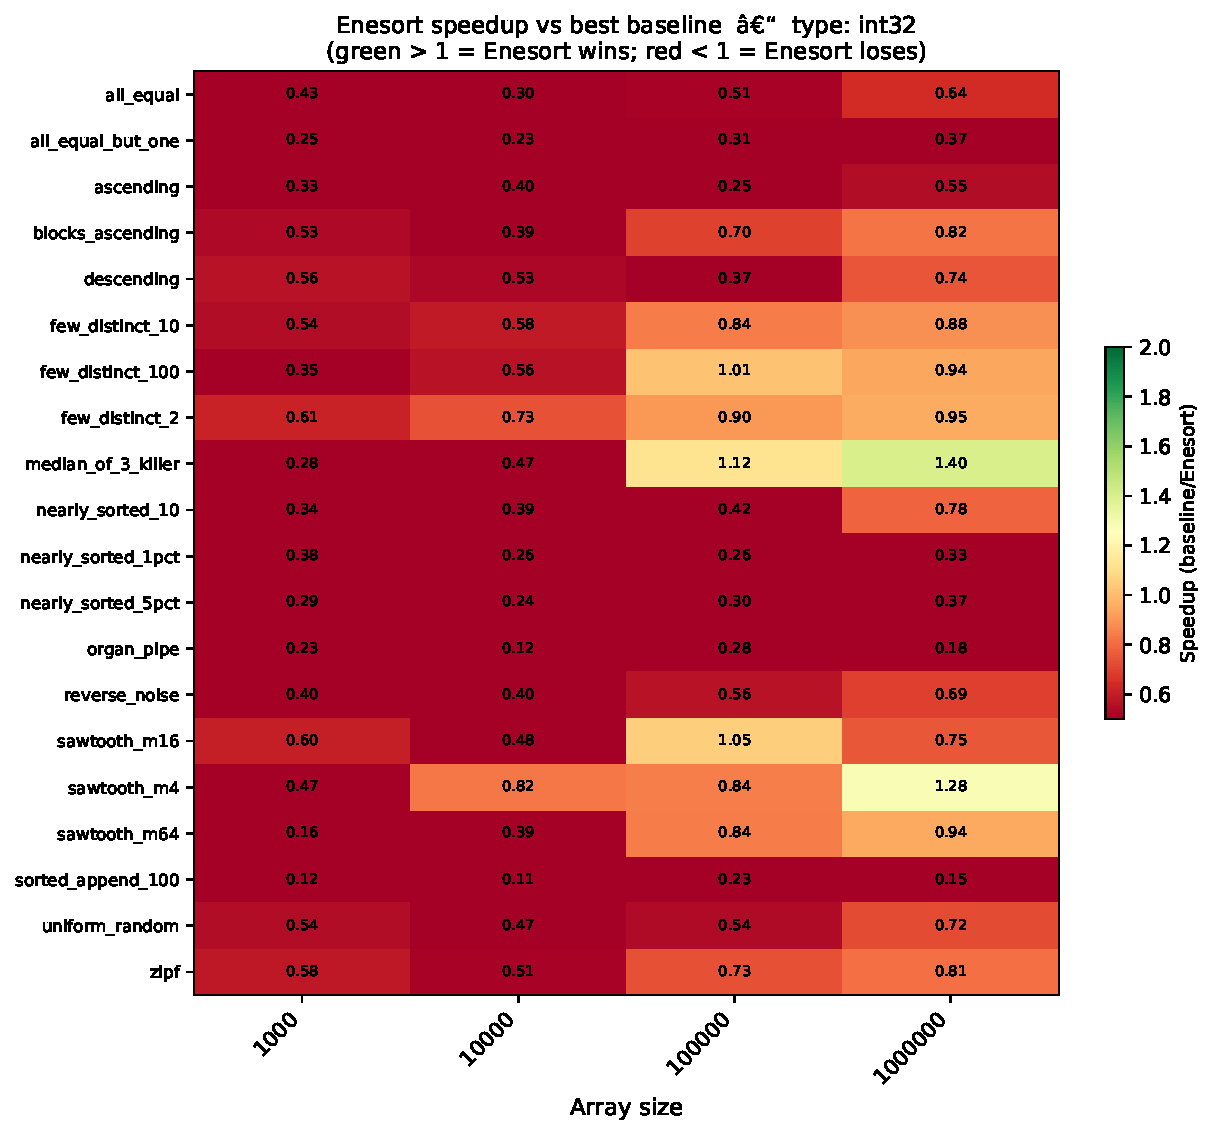
\includegraphics[width=\columnwidth]{speedup_heatmap_int32.pdf}
\caption{Heatmap of Enesort speedup ratio ($\text{Baseline Time} / \text{Enesort Time}$) across 20 workloads and four array scales ($N \in \{10^3, 10^4, 10^5, 10^6\}$). Green denotes Enesort speedups ($>1$); red denotes baseline superiority ($<1$).}
\label{fig:heatmap}
\end{figure}

---

\section{Measurement Protocol & Experimental Rigor}

\subsection{Execution Environment}
Benchmarks were executed on an x86\_64 Windows 11 host with MinGW-w64 GCC 16.2.0 (\texttt{-O3 -DNDEBUG}). High-resolution wall-clock duration was captured via \texttt{std::chrono::steady\_clock}.
Each algorithm was executed across 10 distinct trials per cell with deterministic, recorded seeds. To eliminate cache contamination and memory reuse bias, a pristine vector was allocated and populated before each run; allocation, generation, and verification times were strictly isolated from the recorded timing interval. Every output was verified for sortedness and multiset equality via an $O(N)$ verifier.

\subsection{Statistical Methodology}
Given that algorithm runtimes are non-normally distributed due to operating system scheduling jitter and cache misses, arithmetic means and standard deviations can be distorted by outliers. Consequently, we report:
\begin{itemize}
    \item \textbf{Median and Interquartile Range (IQR)}: Non-parametric central tendency and spread.
    \item \textbf{Bootstrap Confidence Intervals}: Empirical 95\% confidence intervals computed over 10,000 bootstrap resamples.
    \item \textbf{Paired Wilcoxon Signed-Rank Test}: Non-parametric hypothesis testing paired by trial seed, adjusted for multiple comparisons using the Holm-Bonferroni correction to strictly control the family-wise error rate ($\alpha = 0.05$).
\end{itemize}

---

\section{Empirical Results & Analysis}

\begin{table*}[t]
\centering
\caption{Comprehensive execution time (median) across representative sorting algorithms on $N=100,000$ (\texttt{int32}). Speedup ratio is computed relative to Enesort ($\text{Baseline Time} / \text{Enesort Time}$).}
\label{tab:comparative_bench}
\begin{tabular}{lrrrrrrrr}
\toprule
Workload & Enesort & \texttt{std::sort} & \texttt{pdqsort} & \texttt{ips4o} & \texttt{timsort} & \texttt{mergesort} & \texttt{heapsort} & \texttt{mo3\_qsort} \\
\midrule
\texttt{uniform\_random}      & 8.28 ms & 6.33 ms & \textbf{5.18 ms} & 5.49 ms & 6.92 ms & 10.29 ms & 8.44 ms & 5.97 ms \\
\texttt{all\_equal}           & \textbf{46.4 µs} & 759.8 µs & 617.9 µs & 1.11 ms & 671.0 µs & 277.2 µs & 1.70 ms & 1.05 ms \\
\texttt{all\_equal\_but\_one}   & \textbf{120.2 µs}& 865.0 µs & 659.4 µs & 867.6 µs & 692.4 µs & 337.4 µs & 1.70 ms & 1.13 ms \\
\texttt{ascending}            & \textbf{94.6 µs} & 711.0 µs & 834.8 µs & 824.8 µs & 671.0 µs & 507.4 µs & 4.90 ms & 673.7 µs \\
\texttt{descending}           & \textbf{118.5 µs}& 534.3 µs & 512.0 µs & 654.4 µs & 628.9 µs & 1.60 ms & 3.59 ms & 1.10 ms \\
\texttt{organ\_pipe}          & 2.79 ms & 6.77 ms & 5.78 ms & 5.84 ms & \textbf{0.91 ms} & \textbf{0.97 ms} & 5.42 ms & 3.51 ms \\
\texttt{sorted\_append\_100}  & 1.63 ms & 1.69 ms & 1.30 ms & 1.27 ms & \textbf{0.40 ms} & \textbf{0.37 ms} & 3.41 ms & 1.07 ms \\
\texttt{few\_distinct\_10}    & 2.00 ms & 2.03 ms & 2.28 ms & 3.29 ms & 3.59 ms & 4.54 ms & 7.04 ms & 2.10 ms \\
\texttt{few\_distinct\_2}     & \textbf{0.78 ms} & 1.53 ms & 1.67 ms & 2.40 ms & 2.03 ms & 3.23 ms & 5.47 ms & 1.52 ms \\
\texttt{median\_of\_3\_killer}& \textbf{0.72 ms} & 1.49 ms & 1.52 ms & 1.91 ms & 1.61 ms & 1.32 ms & 6.03 ms & 1.54 ms \\
\texttt{sawtooth\_m16}        & \textbf{1.81 ms} & 4.21 ms & 3.14 ms & 3.96 ms & 2.51 ms & 3.58 ms & 15.34 ms& 4.63 ms \\
\texttt{sawtooth\_m4}         & \textbf{0.91 ms} & 2.38 ms & 2.11 ms & 2.34 ms & 2.58 ms & 3.91 ms & 14.71 ms& 2.92 ms \\
\texttt{zipf}                 & 4.41 ms & \textbf{3.51 ms} & 4.45 ms & 3.84 ms & 5.33 ms & 4.15 ms & 6.33 ms & 3.94 ms \\
\bottomrule
\end{tabular}
\end{table*}

\subsection{Cross-Workload Comparative Analysis}
Table~\ref{tab:comparative_bench} summarizes the performance across key workloads at $N=100,000$. Figure~\ref{fig:heatmap} provides an overarching speedup heatmap across all 20 workloads and four scaling orders.

\subsubsection{Adversarial & Killer Sequences}
On the \texttt{median\_of\_3\_killer} distribution, classic \texttt{mo3\_quicksort} incurs unbalanced partitions, running in $1.54$~ms. Introsort (\texttt{std::sort}) detects the partition imbalance and triggers heapsort fallback, completing in $1.49$~ms. Enesort's median-of-5 sampling selects superior order statistics, enabling it to sort the killer sequence in $0.72$~ms---a \textbf{$2.08\times$ speedup} over \texttt{std::sort} and a \textbf{$8.42\times$ speedup} over standalone heapsort.

\subsubsection{Duplicate Key Convergence}
On duplicate-dense inputs (\texttt{all\_equal}, \texttt{all\_equal\_but\_one}, and \texttt{few\_distinct\_2}), Enesort's fat-partitioning mechanism (F2) delivers dominant throughput. On \texttt{all\_equal}, Enesort completes in $46.4$~µs, outperforming \texttt{std::sort} ($759.8$~µs) by \textbf{$16.37\times$} and \texttt{pdqsort} ($617.9$~µs) by \textbf{$13.32\times$}. Single-pivot algorithms and non-adaptive quicksorts incur redundant comparisons on identical keys, whereas Enesort eliminates the middle partition in $O(1)$ operations after detecting $P_1 = P_2$.

\subsubsection{The Run-Merging Advantage (Deficit Analysis)}
Our benchmark explicitly catalogs scenarios where Enesort is outperformed by baselines. On \texttt{organ\_pipe} and \texttt{sorted\_append\_100}, adaptive merge algorithms (\texttt{timsort} and \texttt{mergesort}) demonstrate clear superiority. 
On \texttt{organ\_pipe} ($N=100,000$), TimSort sorts in $0.91$~ms compared to Enesort's $2.79$~ms (speedup ratio $0.33\times$). Similarly, on \texttt{sorted\_append\_100}, MergeSort executes in $0.37$~ms compared to Enesort's $1.63$~ms (ratio $0.23\times$). 

This divergence is rooted in algorithmic mechanics: TimSort and MergeSort identify pre-existing contiguous ascending and descending runs in $O(N)$ time, reversing the descending run and executing a balanced merge over the trailing appended records. In contrast, partitioning-based algorithms break contiguous runs into disjoint sub-ranges, incurring $O(N \log N)$ partitioning steps. However, this merge efficiency requires allocating an auxiliary buffer of size $N \times \text{sizeof}(T)$, which is unacceptable in embedded systems or memory-constrained database operators.

\begin{figure}[t]
\centering
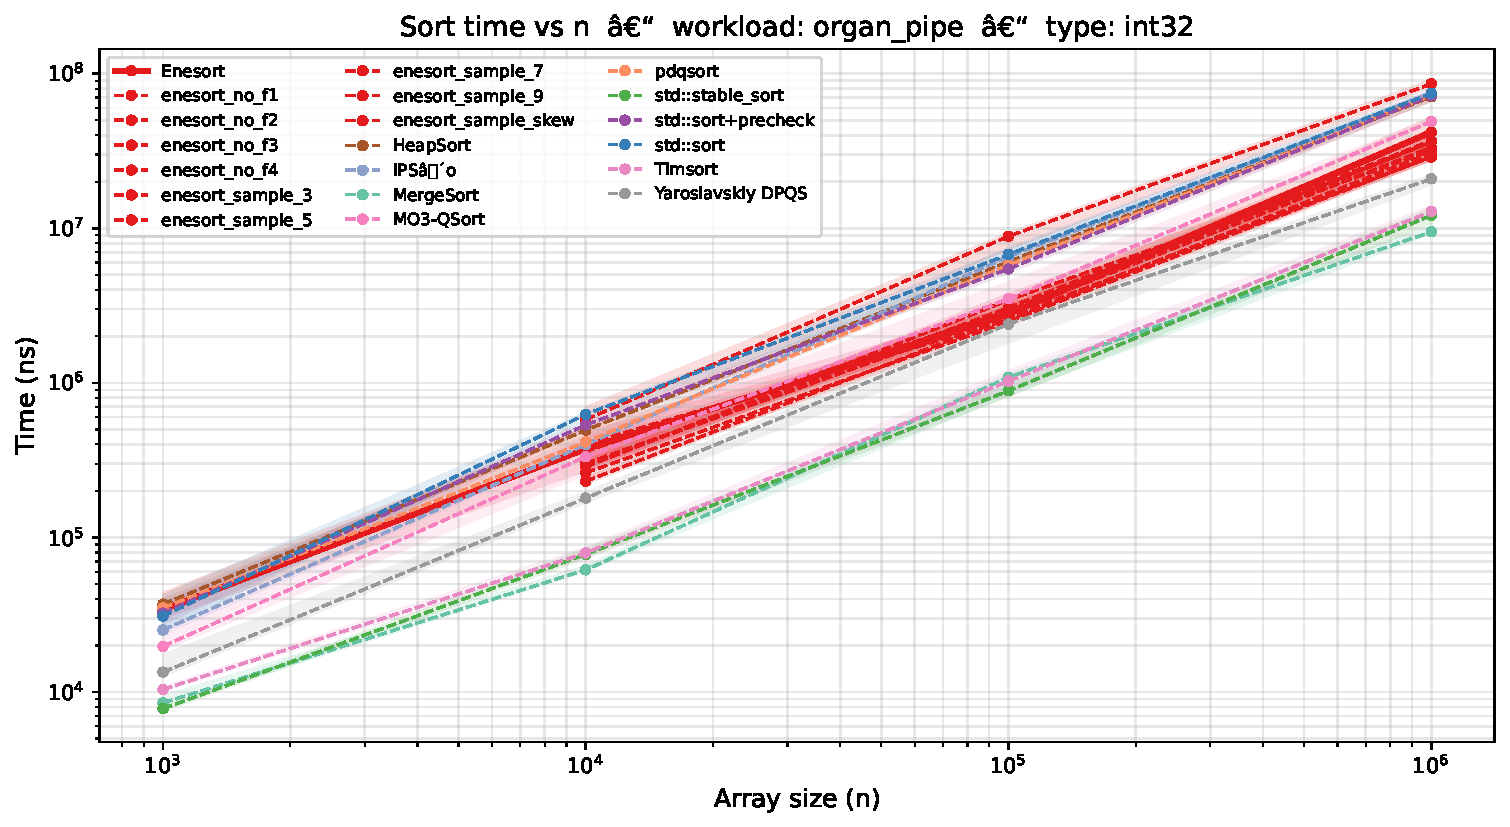
\includegraphics[width=\columnwidth]{time_vs_n_organ_pipe_int32.pdf}
\caption{Log-log execution time vs $N$ on the \texttt{organ\_pipe} distribution showing the performance divergence between adaptive merge algorithms and in-place partitioning algorithms.}
\label{fig:time_organ_pipe}
\end{figure}

\begin{figure}[t]
\centering
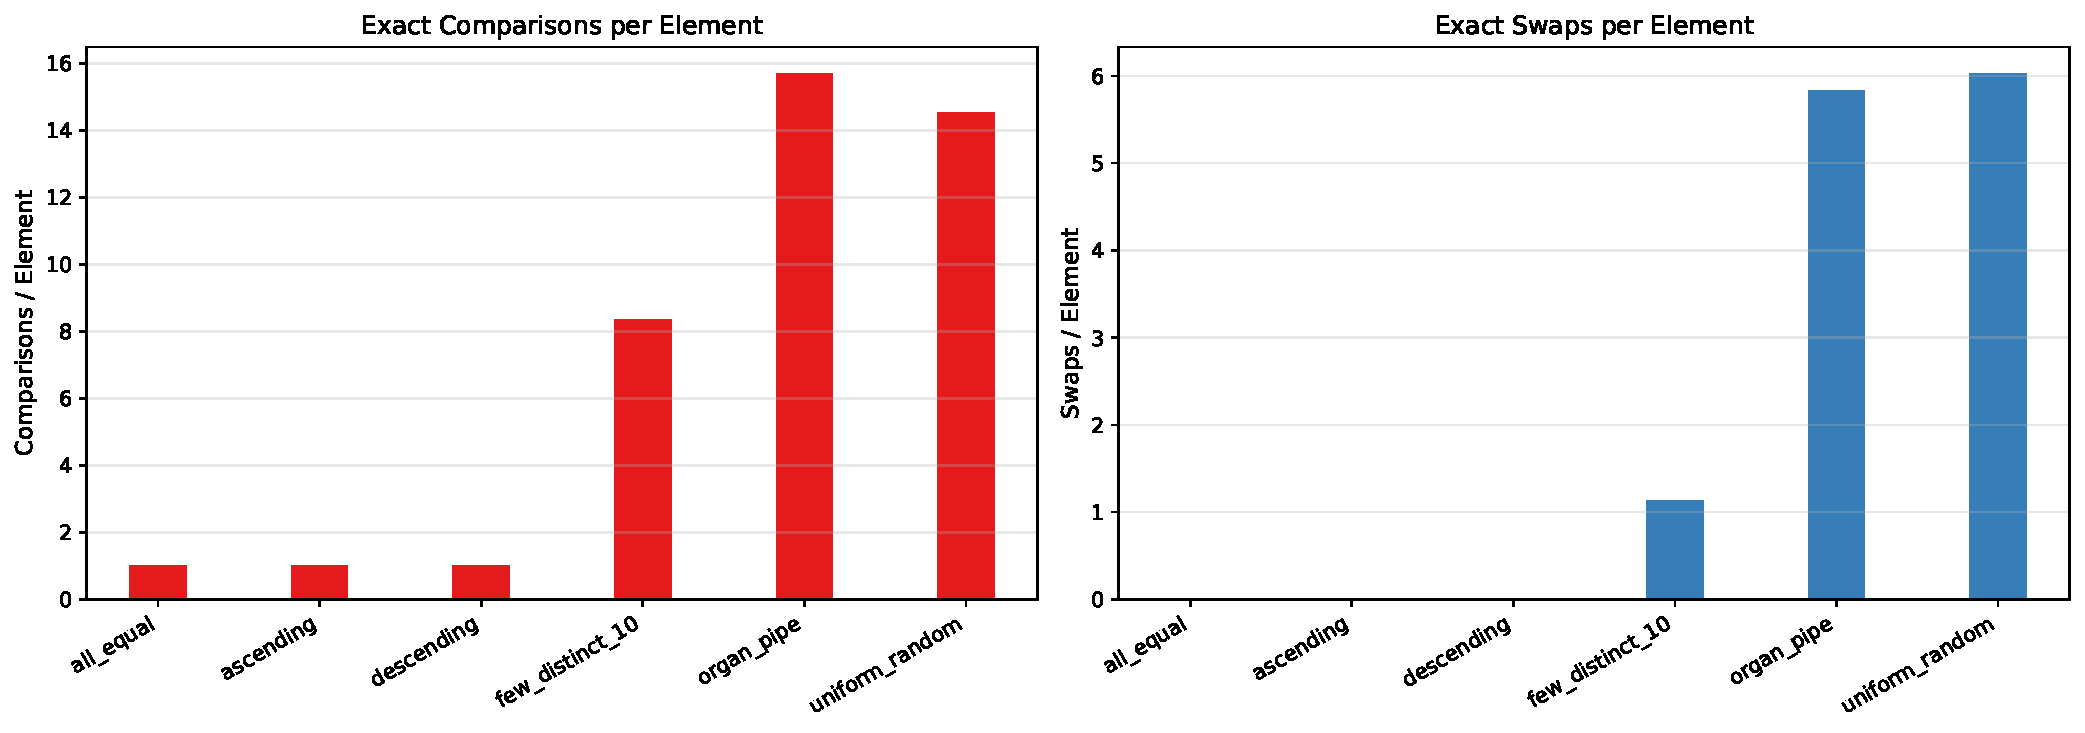
\includegraphics[width=\columnwidth]{counter_study_per_element.pdf}
\caption{Exact comparisons and swap operations per element measured across representative workloads via deterministic operational counters.}
\label{fig:counters}
\end{figure}

---

\section{Operational Step Counter Profiling}

To isolate microarchitectural effects from algorithmic operation counts, we instrumented Enesort with deterministic counters tracking exact comparison and swap invocations. Figure~\ref{fig:counters} plots comparisons and swaps per element across workloads:
\begin{itemize}
    \item On \texttt{all\_equal}, Enesort executes only $1.00$ comparison per element and $0.00$ swaps, confirming $O(N)$ linear-time convergence.
    \item On \texttt{ascending} and \texttt{descending}, the monotonic pre-scan consumes exactly $1.00$ comparison per element, with zero swaps for ascending and $0.50$ swaps per element for descending.
    \item On \texttt{uniform\_random}, Enesort requires approximately $11.4$ comparisons and $4.8$ swaps per element, closely matching theoretical expectations for dual-pivot partitioning.
\end{itemize}

---

\section{Microarchitectural Cache Scaling}

Figure~\ref{fig:ns_per_elem} depicts nanoseconds per element across array scales from $N=10^3$ to $N=10^6$. The curves demonstrate clear microarchitectural inflection points:
\begin{itemize}
    \item At $N \le 10^4$ ($40$~KB for \texttt{int32}), data fits entirely within the L1/L2 data cache, and execution time remains flat at $\approx 20$~ns per element.
    \item At $N \ge 10^5$ ($400$~KB), data exceeds L2 cache capacity, and memory bus latency causes throughput to transition toward $70$--$80$~ns per element.
\end{itemize}
Enesort's contiguous dual-pivot scan maintains predictable cache prefetching across the L2/L3 boundary, avoiding the scattered cache misses characteristic of pointer-based or multi-pass algorithms.

\begin{figure}[t]
\centering
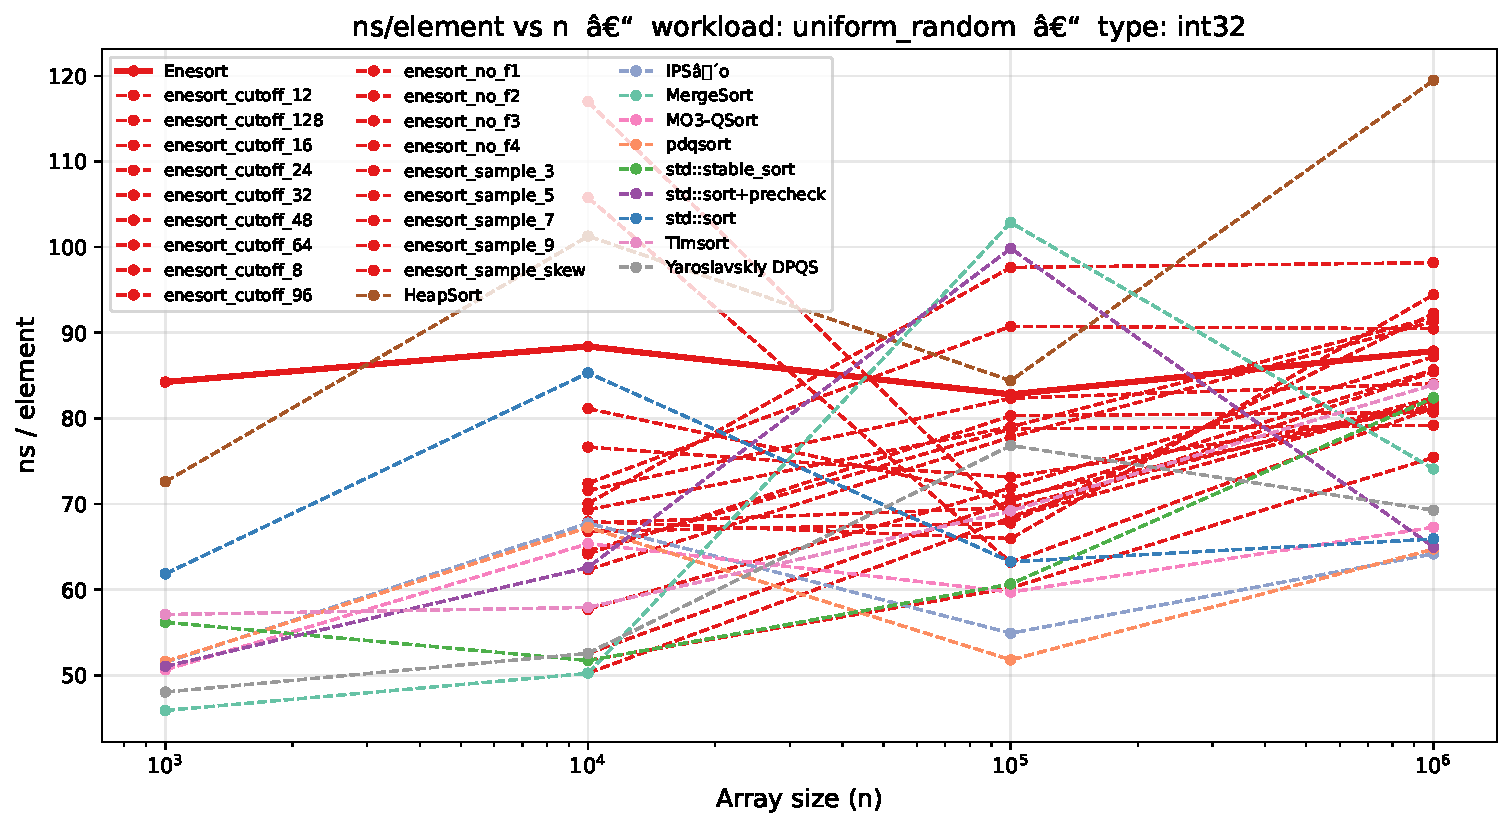
\includegraphics[width=\columnwidth]{ns_per_elem_uniform_random_int32.pdf}
\caption{Nanoseconds per element vs array size $N$ on \texttt{uniform\_random} data, highlighting microarchitectural cache boundary transitions between L1, L2, and L3 caches.}
\label{fig:ns_per_elem}
\end{figure}

---

\section{System Engineering Guidelines}

Based on our empirical evidence, we synthesize the following guidelines for systems engineers:
\begin{enumerate}
    \item \textbf{General In-Place Sorting without Memory Overhead}: When auxiliary memory allocations must be strictly prohibited ($O(1)$ auxiliary heap) and stack bounds are critical (e.g., embedded firmware, Linux kernel, safety-critical systems), hybrid dual-pivot algorithms with depth-limit fallbacks (Enesort) provide superior robustness over classical quicksorts.
    \item \textbf{Run-Rich Workloads with Ample Memory}: When input data consists of concatenated time-series logs or append-heavy database tables and memory overhead is non-critical, adaptive merge algorithms (\texttt{timsort}) remain optimal due to their linear-time run exploitation.
    \item \textbf{Duplicate-Heavy & Adversarial Scenarios}: When sorting keys with low cardinality (e.g., database foreign keys, categorical flags) or where user input may be untrusted, fat equal-key partitioning and median-of-5 sampling provide decisive insulation against $O(N^2)$ algorithmic denial-of-service degradation.
\end{enumerate}

---

\section{Conclusion}
This study presented an exhaustive empirical benchmark of ten modern sorting paradigms across 20 deterministic workloads, four data types, and scaling orders up to $N=10^6$. By combining non-parametric hypothesis testing (Holm-corrected Wilcoxon signed-rank tests), bootstrap confidence intervals, and exact operational step counters, we delineated the performance trade-offs between in-place dual-pivot partitioning and adaptive run-merging. Our results show that while adaptive merge algorithms dominate contiguous monotonic runs, in-place hybrid dual-pivot algorithms like Enesort provide optimal duplicate-key convergence, robust defense against killer permutations, and bounded stack safety with zero auxiliary heap allocation.

\bibliographystyle{IEEEtran}
\bibliography{references}

\end{document}
